\documentclass[tikz,border=10pt]{standalone}
\usepackage{tikz}
\usetikzlibrary{positioning,arrows.meta,shapes,calc,shadows}

\begin{document}
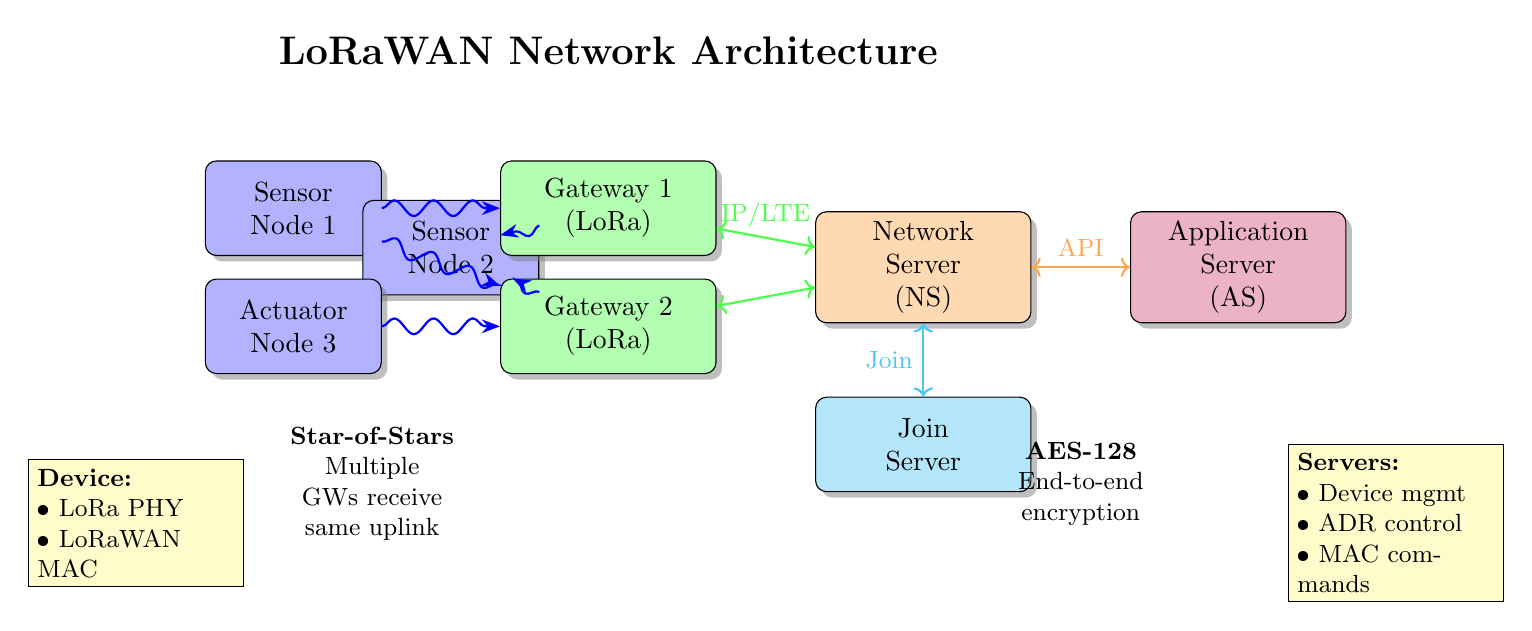
\begin{tikzpicture}[
    device/.style={rectangle, draw, fill=blue!30, text width=2cm, text centered, rounded corners, minimum height=1.2cm, drop shadow},
    gateway/.style={rectangle, draw, fill=green!30, text width=2.5cm, text centered, rounded corners, minimum height=1.2cm, drop shadow},
    server/.style={rectangle, draw, fill=orange!30, text width=2.5cm, text centered, rounded corners, minimum height=1.2cm, drop shadow},
    app/.style={rectangle, draw, fill=purple!30, text width=2.5cm, text centered, rounded corners, minimum height=1.2cm, drop shadow},
    arrow/.style={-Stealth, thick},
    wireless/.style={decorate, decoration={snake, amplitude=1mm, segment length=5mm}},
]

% Title
\node[font=\Large\bfseries] at (0,8) {LoRaWAN Network Architecture};

% End Devices
\node[device] (dev1) at (-4,6) {Sensor\\Node 1};
\node[device] (dev2) at (-2,5.5) {Sensor\\Node 2};
\node[device] (dev3) at (-4,4.5) {Actuator\\Node 3};

% Gateways
\node[gateway] (gw1) at (0,6) {Gateway 1\\(LoRa)};
\node[gateway] (gw2) at (0,4.5) {Gateway 2\\(LoRa)};

% Network Server
\node[server] (ns) at (4,5.25) {Network\\Server\\(NS)};

% Application Server
\node[app] (as) at (8,5.25) {Application\\Server\\(AS)};

% Join Server
\node[server, fill=cyan!30] (js) at (4,3) {Join\\Server};

% Connections - Devices to Gateways (wireless)
\draw[arrow, blue, wireless] (dev1) -- (gw1);
\draw[arrow, blue, wireless] (dev1) -- (gw2);
\draw[arrow, blue, wireless] (dev2) -- (gw1);
\draw[arrow, blue, wireless] (dev2) -- (gw2);
\draw[arrow, blue, wireless] (dev3) -- (gw2);

% Connections - Gateways to Network Server
\draw[arrow, green!70, <->] (gw1) -- node[above, font=\small] {IP/LTE} (ns);
\draw[arrow, green!70, <->] (gw2) -- (ns);

% Connection - Network Server to Application Server
\draw[arrow, orange!70, <->] (ns) -- node[above, font=\small] {API} (as);

% Connection - Network Server to Join Server
\draw[arrow, cyan!70, <->] (ns) -- node[left, font=\small] {Join} (js);

% Annotations
\node[font=\small, text width=3cm, align=center] at (-3,2.5) {
    \textbf{Star-of-Stars}\\
    Multiple GWs receive\\
    same uplink
};

\node[font=\small, text width=3cm, align=center] at (6,2.5) {
    \textbf{AES-128}\\
    End-to-end\\
    encryption
};

% Protocol layers
\node[font=\small, text width=2.5cm, align=left, draw, fill=yellow!20] at (-6,2) {
    \textbf{Device:}\\
    • LoRa PHY\\
    • LoRaWAN MAC
};

\node[font=\small, text width=2.5cm, align=left, draw, fill=yellow!20] at (10,2) {
    \textbf{Servers:}\\
    • Device mgmt\\
    • ADR control\\
    • MAC commands
};

\end{tikzpicture}
\end{document}
